\documentclass[a4paper]{article}

%%%%%%%%%%%%%%%%
%%% PREAMBLE %%%
%%%%%%%%%%%%%%%%

%%% PACKAGES %%%
\usepackage{fontspec}                     % set fonts
	\setmainfont{Junicode}
\usepackage[a4paper,margin=3cm]{geometry} % page layout
\usepackage[svgnames]{xcolor}             % rainbowssss *_*
\usepackage{hyperref}                     % enhanced references (links)
	\hypersetup{%
		colorlinks=true,
		allcolors=NavyBlue}
\usepackage{fancyhdr}                     % headers & footers
\usepackage{titling}                      % macros \thetitle, \theauthor
\usepackage{graphicx}                     % enhanced graphics support
	\graphicspath{{img/}}
\usepackage[toc]{glossaries}              % glossaries (obv)
	\setglossarystyle{altlisthypergroup}
	\makeglossaries
	\newglossaryentry{turnstile}
{%
	name=turnstile,
	description={An ingress control device to help with the organizization
	of the passengers’ boarding. Basically a lockable revolving gate with
	three arms. When signalled, the gate unlocks and a single passenger may
	go through by turning one of the arms. After a single rotation, the gate
	locks again, waiting for the next signal.}
}

\newglossaryentry{authentication}
{%
	name=authentication,
	description={The process of verifying the \textit{identity} of the
	passengers.}
}

\newglossaryentry{authorization}
{%
	name=authorization,
	description={The process of veryfying whether an identified passenger
	has \textit{permission} to do something (eg board the bus).}
}

\newglossaryentry{alarm}
{%
	name=alarm,
	description={A device installed at every door that emits light and sound
	to draw attention to certain events. For instance, it signals the end of
	the boarding phase and also turns on in the event of an unauthorized
	boarding attempt.}
}

\newglossaryentry{RFIDScanner}
{%
	name={RFID scanner},
	description={An instrument capable of reading radio frequency
	identification tags. This can be used to effectively identify
	passengers.}
}

\newglossaryentry{boardingController}
{%
	name={boarding controller},
	description={A device responsible for the orchestration of the whole
	boarding phase (signalling doors to open or close, activating the alarm,
	etc).}
}

\usepackage{enumitem}                     % enhanced enumerations
\usepackage{tabularx}                     % enhanced tables
\usepackage{float}                        % 'H' figure placement
\usepackage{rotating}                     % sidewaysfigure
\usepackage[noabbrev]{cleveref}           % clever references
\usepackage{booktabs}                     % pretty tables

%%% OTHER %%%
\setlength\headheight{22.3725pt}

%%% META %%%
\title{Assignment \#1 \\ Requirement analysis}
\author{Levendula}
\date{\today}

%%% ADDITIONAL PACKAGE CONFIG %%%
% fancyhdr
\pagestyle{fancy}
\fancyhf{}
\lhead{\theauthor}
\rhead{\thetitle}
\lfoot{\today}
\rfoot{\thepage}

%%%%%%%%%%%%%%%%%%%%%%%%%%%%%%%%%%%%%%%%%%%%%%%%%%%%%%%%%%%%%%%%%%%%%%%%%%%%%%%%

%%%%%%%%%%%%
%%% BODY %%%
%%%%%%%%%%%%

\begin{document}

\begin{titlepage}
	\begin{center}
		
\includegraphics[width=8cm]{logo.jpg}

		\vspace{.2cm}

		\textbf{Budapest University of Technology and Economics} \\
		Faculty of Electrical Engineering and Informatics \\
		Department of Measurement and Information Systems \\

		\vspace{2cm}

		{\huge IT System Design (\texttt{VIMIAC01})}

		\vspace{2cm}

		{\huge \bfseries \thetitle}

		\vspace{.5cm}

		{\Large \theauthor}

		\vspace{.5cm}

		{\Large \today}
	\end{center}

	\vfill{}

	{\large Team members:}

	\vspace{.25cm}

	\begin{tabular}{lll}
		Annamária Gálik &
			\texttt{WGMUO2} &
			ancsi666@gmail.com \\
		Borbála Szilágyi &
			\texttt{COVQ1M} &
			szilagyiborbala8@gmail.com \\
		Bertalan Z. Péter &
			\texttt{QO7CU6} &
			bertalan.peter+uni@bertalanp99.eu
	\end{tabular}

	\vspace{2cm}
\end{titlepage}


\tableofcontents
\listoffigures
\clearpage

% ------------------------------------------------------------------------------
\section{Our task}

% Ancsi: Nem kell a dolgokat {} közé tenni, csak ritkán (akkor, ha alkalmazni
% akarsz rájuk valami olyan makrót, ami ilyen blokkokra teljesül, pl \scriptsize
% (de ilyet csak kivételes esetekben csinálunk)
% A sorok végére sem kell tenni \\-t, hanem egy sort kihagyva érjük el, hogy új
% paragrafus legyen
% -- Berci

Our job was to do the preparation of installing \gls{driverless}
\gls{autonomous} \gls{vehicle}s in order to offer \gls{transportation} service
to the workers at a private office park.

We had to identify the \gls{stakeholder}s, model the context of the planned
system, and also to define the high-level requirements, necessary functions and
use cases. We also documented non-trivial terms in a glossary as well as the
ambiguous or contradicting requirements so as to be able to contact the customer
with well-defined questions.

We were to study the appendices, which arose some new questions that we
discussed.


% ------------------------------------------------------------------------------
\section{Ambiguities and our ideas}

\begin{enumerate}
	\item Interpretation of ‘make sure the buses are not overcrowded’

		\textit{The buses form a network that is capable of
			intelligently deciding which bus to ‘send’ where, in
			accordance to the number of people \gls{request}ing the
			bus at the \gls{terminal}s, what \gls{route}s other
			buses have planned, and how many people are on certain
			buses. Overcrowding can be avoided provided there is a
			sufficient number of \gls{vehicle}s at our disposal and
			the buses can \gls{autonomous}ly decide their
			\gls{route}s in such a way that no single bus is full
			while others are on low capacity. Essentially, we could
			balance the number of passengers on the buses.}

	\item What does a \gls{request} contain? Who can publish a
	      \gls{request}?

		\textit{The \gls{request} must contain the indentification of
			the worker who ordered the bus, the number of passengers
			who will travel, the starting point, the destination,
			and the planned time of the trip. Requests can be made
			from the installed terminals by anybody—this does not
			introduce a problem, since the system operates inside a
			closed-off, private office park—but in order to use
			the \gls{mobileApplication}, registration is needed.}

	\item Can passengers change their destination during the trip?

		\textit{Passengers should not be able to select new
			destionations after they already boarded on of the
			buses. Should a passenger need to abort their current
			trip and travel somewhere else for whatever reason, they
			are urged to get off anywhere where the bus would
			normally stop and \gls{request} a new lift from there.}
\end{enumerate}


% ------------------------------------------------------------------------------
\section{List of stakeholders}

See~\cref{fig:stakeholders} for a diagram describing the relations of these
\gls{stakeholder}s.

\begin{description}[style=nextline]%,align=right,leftmargin=6cm]
	\item[authorities]
		A body of persons having power to make and enforce law.

	\item[office workers]
		The people working at the client's company; the main users of
		the \gls{autonomous} buses.

	\item[Health\&Safety Department]
		A group at our company responsible for analyzing the
		potential health and safety risks of our products and
		forming rules and regulations to make sure these risks
		are averted.

	\item[project sponsor]
		An single person who holds overall responsibilty for the
		project's success. They are \emph{not} to manage the day-to-day
		operations but to promote the project and provide the necessary
		resources.

	\item[project manager]
		A person who takes responsibility for the planning, preparation,
		and execution of the project. They are responsible for
		accomplishing the project's objectives.

	\item[architects]
		People skilled in the area of planning and various physical
		structures. Our waiting areas near the office buildings shall be
		planned by them.

	\item[\gls{autonomous} \gls{vehicle} control engineers]
		They are capable of developing new technologies and handling
		problems of \gls{autonomous} \gls{vehicle} transport systems
		taking into account environmental and energy management
		requirements.

	\item[mechanical engineers]
		Engineers specialized in working with automotive mechanical
		systems, such as the buses themselves.

	\item[software developers]
		They create, maintain and implement computer software.

	\item[system testers]
		A group that creates testing plans for the system and identifies
		what parts of a system can be tested using \gls{automated} tools
		and what require manual testing. This team is also responsible
		for running the tests.

	\item[mechanics]
		People who repair and maintain machinery.

	\item[suppliers]
		The organizations that provide needed elements, products, and
		services for the project.

	\item[our company’s management]
		The group of people in charge of our company.

	\item[client's management]
		The group of people in charge of our client's company.
\end{description}

\begin{figure}
	\centering
	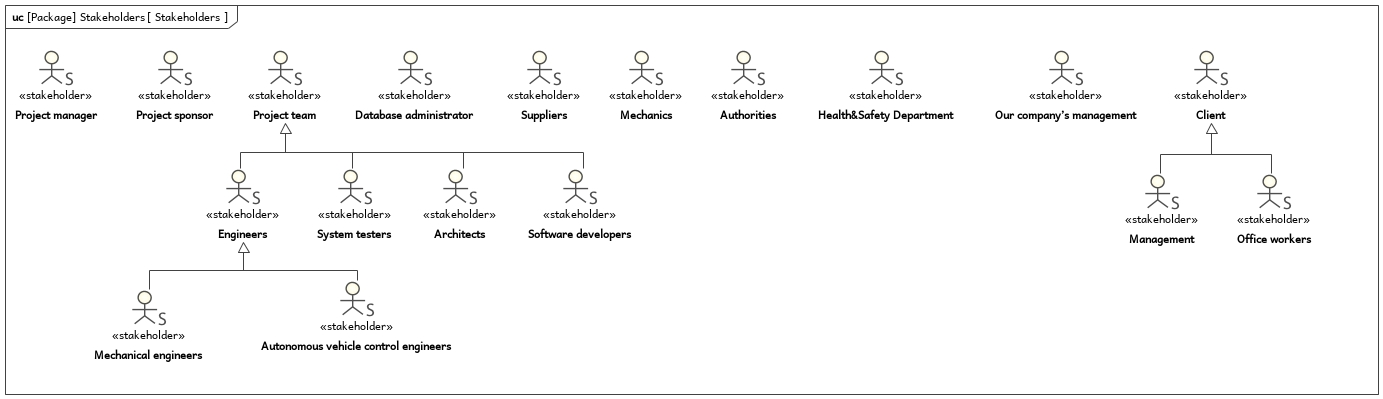
\includegraphics[width=\textwidth]{stakeholders.jpg} % TODO ugly
	\caption{Diagram of stakeholders}%
	\label{fig:stakeholders}
\end{figure}



% ------------------------------------------------------------------------------
\section{System context}

\begin{figure}[H]
	\centering
	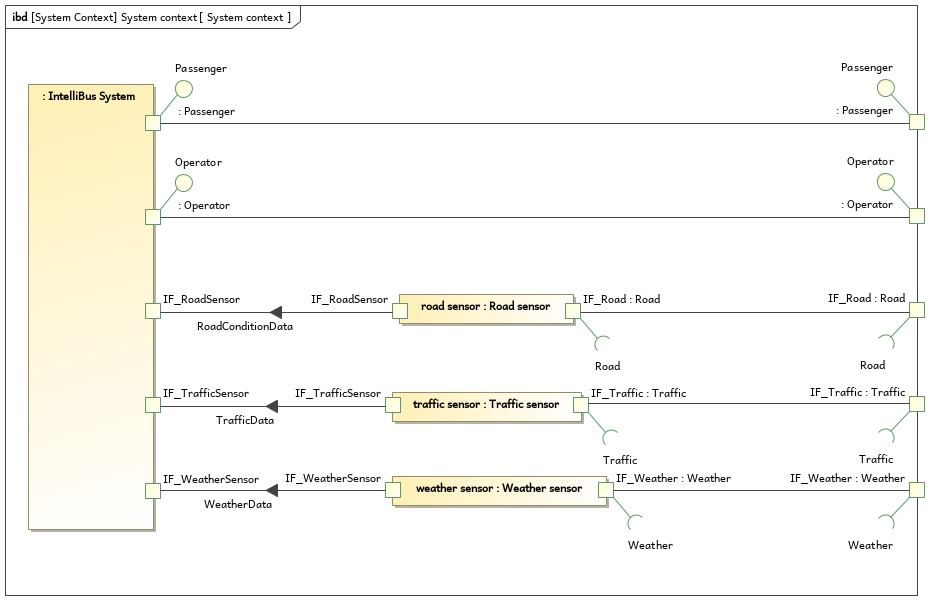
\includegraphics[width=\textwidth]{context.jpg}
	\caption{System Context diagram}
\end{figure}


% ------------------------------------------------------------------------------
\section{Requirements}

See figures~\crefrange{fig:req-functional}{fig:req-usability} for a visual
representation of these requirements.

\subsection{Functional requirements}
\begin{tabularx}{\textwidth}{p{.9cm} X}
	F1     & The buses shall get around \gls{autonomous}ly inside the
	         \gls{site}. \\

	F1.1   & The buses shall be capable of transporting passengers around
	         the office park. \\

	F2.2   & The buses shall select their \gls{route} \gls{automatically}
	         based on the current demand. \\

        F1.3   & The buses must not have any permanent personnel on board. \\

	F2     & The buses shall have a dedicated \gls{station} in the park for
	         storage and maintenance. \\

	F3     & The passengers should be able to publish their
	         \gls{transportation} \gls{request}s. \\

	F3.1   & Registered users should be able to publish their \gls{request}s
	         in advance using a \gls{mobileApplication}. \\

	F3.2   & Passengers should be able to publish their \gls{transportation}
	         \gls{request}s through the \gls{terminal}s. \\

	F3.2.1 & Dedicated \gls{terminal}s should be installed in front of every
	         major office building. \\
\end{tabularx}

\begin{sidewaysfigure}
	\centering
	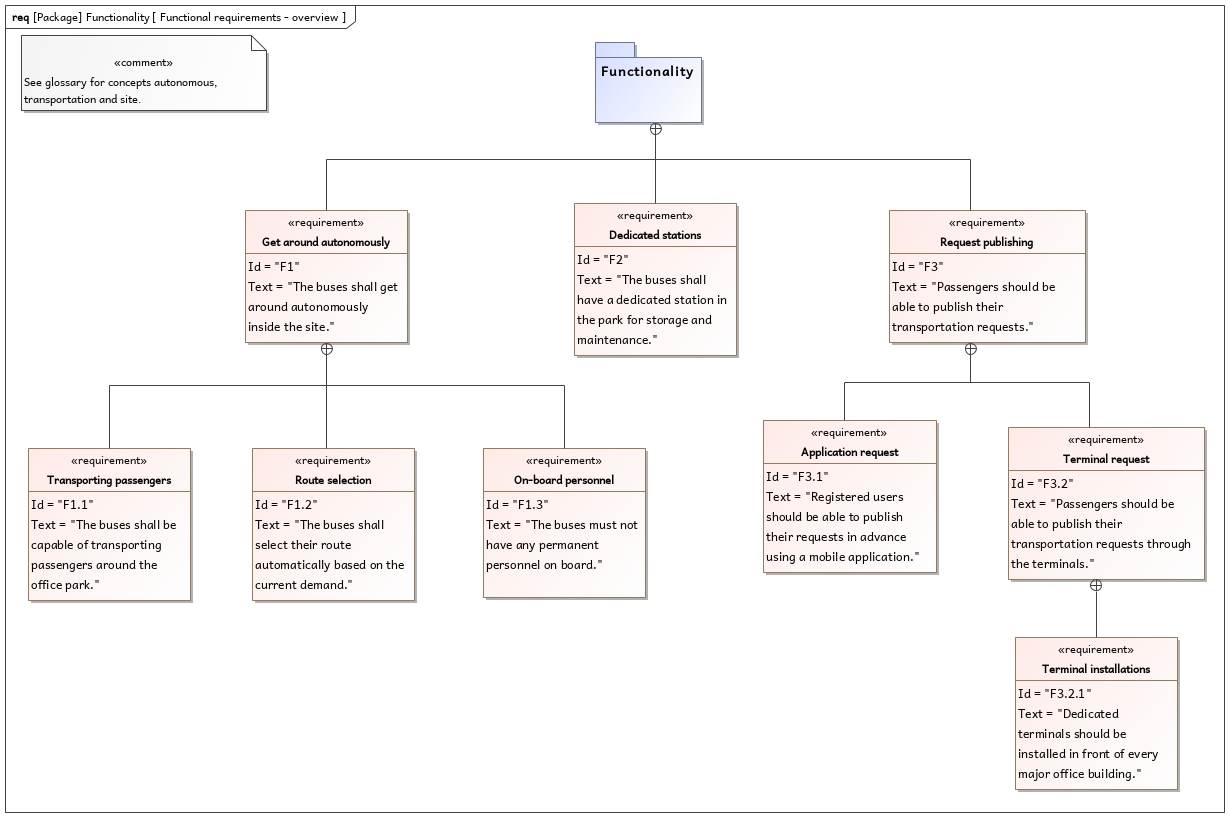
\includegraphics[width=\textwidth]{req-functional.jpg}
	\caption{Functional requirement diagram}%
	\label{fig:req-functional}
\end{sidewaysfigure}

\subsection{Performance requirements}
\begin{tabularx}{\textwidth}{p{.9cm} X}
        P1 & The waiting time for a bus may not exceed 30 minutes. \\
        P2 & The buses shall operate between 7 AM and 10 PM every workday. \\
\end{tabularx}

\begin{figure}
	\centering
	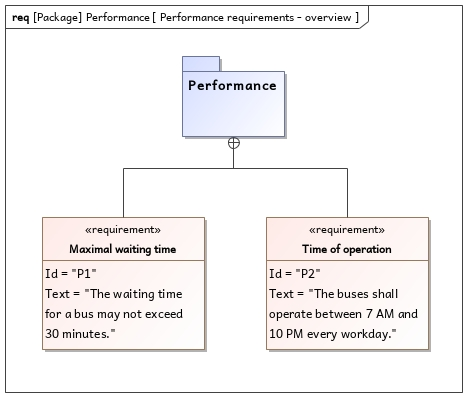
\includegraphics[width=.75\textwidth]{req-performance.jpg}
	\caption{Performance requirement diagram}%
	\label{fig:req-performance}
\end{figure}

\subsection{Reliability requirements}
\begin{tabularx}{\textwidth}{p{.9cm} X}
	R1 & The buses shall be able to complete at least 100 km on average
	     between two interventions. \\

	R2 & At least ⅔ of the buses should be operational at all times. \\

        R3 & The buses should balance their load evenly if possible. \\
\end{tabularx}

\begin{figure}
	\centering
	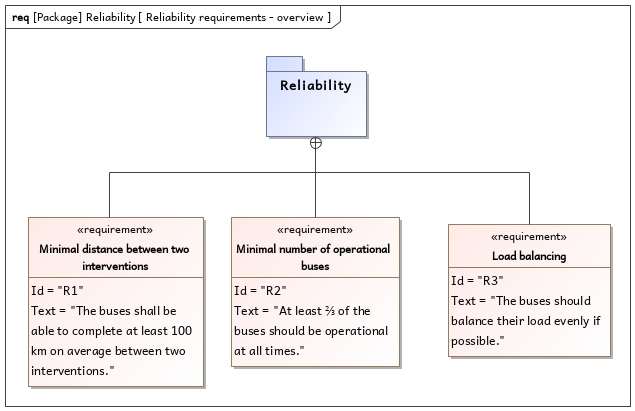
\includegraphics[width=.75\textwidth]{req-reliability.jpg}
	\caption{Reliability requirement diagram}%
	\label{fig:req-reliability}
\end{figure}

\subsection{Safety requirements}
\begin{tabularx}{\textwidth}{p{.9cm} X}
        SA01 & The buses must avoid causing any harm to the passengers. \\

	SA02 & The system should have a database which contains actual
	       information about the condition of the buses. \\

        SA03 & The buses must avoid causing accidents. \\

	SA04 & The buses should be equipped with \gls{sensor}s that can
	       \gls{monitor} road conditions. \\

	SA05 & The buses must successfully complete a 30-day test run before
	       acceptance. \\

        SA06 & The buses may not be overcrowded. \\

        SA07 & Health\&Safety regulations must be fulfilled. \\

        SA08 & The buses may have a \gls{blackBox}. \\

	SA09 & The buses should close their doors only when no passenger is
	       standing in the doorway. \\

	SA10 & The buses should only brake gracefully, except when abrupt
	       braking is the only viable option to avoid an accident. \\

	SA11 & The Health\&Safety Department should have access to the database.
	       \\

	SA13 & The \gls{autonomous} \gls{vehicle}s must be able to react to the
	       behaviour of cyclists and pedestrians. \\
\end{tabularx}

\begin{sidewaysfigure}
	\centering
	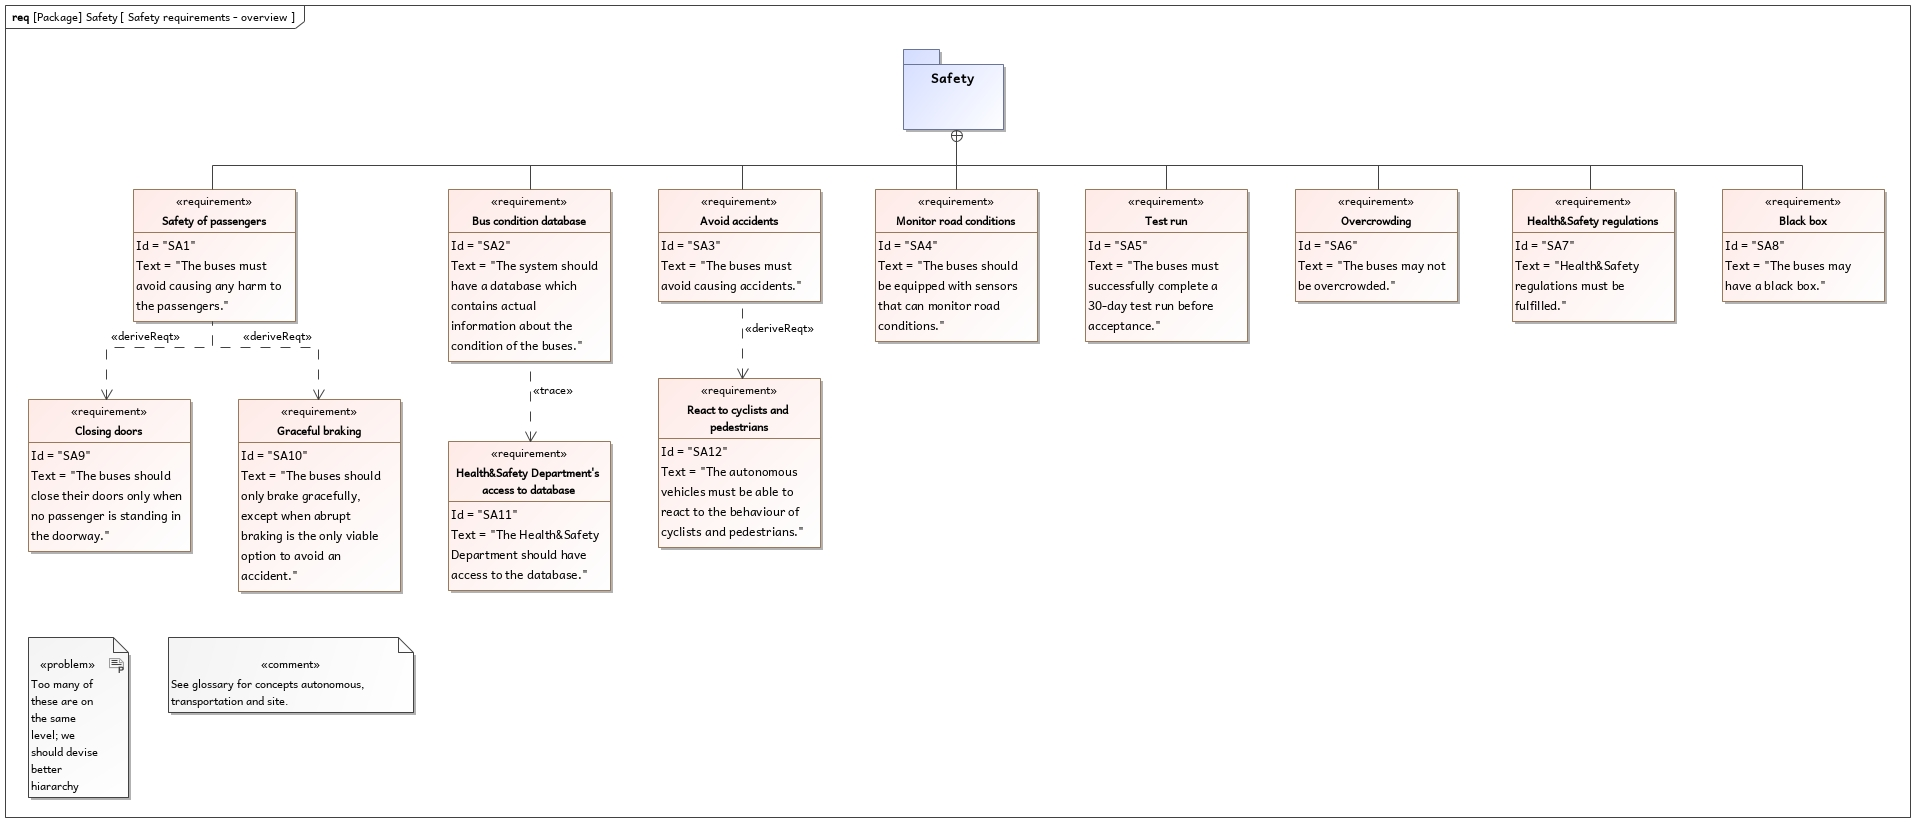
\includegraphics[width=\textwidth]{req-safety.jpg}
	\caption{Safety requirement diagram}%
	\label{fig:req-safety}
\end{sidewaysfigure}

\subsection{Security requirements}
\begin{tabularx}{\textwidth}{p{.9cm} X}
	SE1 & The system must provide control access only to \gls{authorized}
	      personnel. \\

	SE2 & The \gls{mobileApplication} must protect the personal information
	      of the users. \\
\end{tabularx}

\begin{figure}
	\centering
	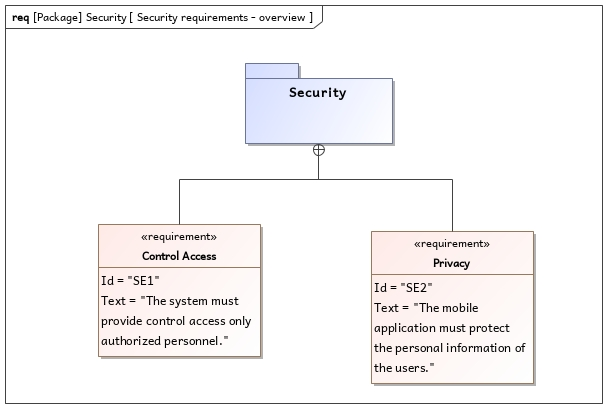
\includegraphics[width=.75\textwidth]{req-security.jpg}
	\caption{Security requirement diagram}%
	\label{fig:req-security}
\end{figure}

\subsection{Supportability requirements}
\begin{tabularx}{\textwidth}{p{.9cm} X}
	SU1 & The buses should be able to notify the maintenance team and return
	      to the \gls{station} \gls{autonomous}ly in case of a
	      \gls{non-criticalFailure}. \\

	SU2 & Buses may have a group of 2–3 people \gls{station}ed on \gls{site}
	      who can intervene (either remotely or manually) in case of a
	      \gls{technicalProblem}. \\
\end{tabularx}

\begin{figure}
	\centering
	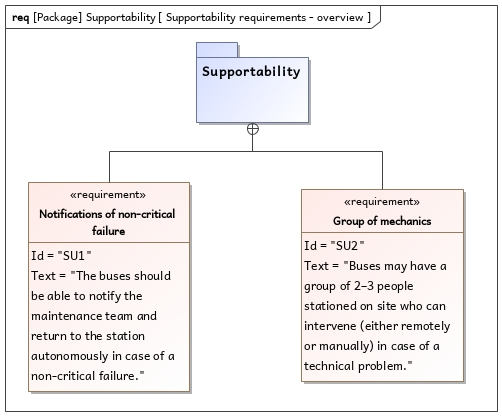
\includegraphics[width=.75\textwidth]{req-supportability.jpg}
	\caption{Supportability requirement diagram}%
	\label{fig:req-supportability}
\end{figure}

\subsection{Usability requirements}
\begin{tabularx}{\textwidth}{p{.9cm} X}
        U1 & The buses must be able to operate under any weather conditions. \\

        U2 & The bus \gls{station}s may be covered. \\

	U3 & The \gls{mobileApplication}’s login screen should be simple and
	     efficient. \\
\end{tabularx}

\begin{figure}
	\centering
	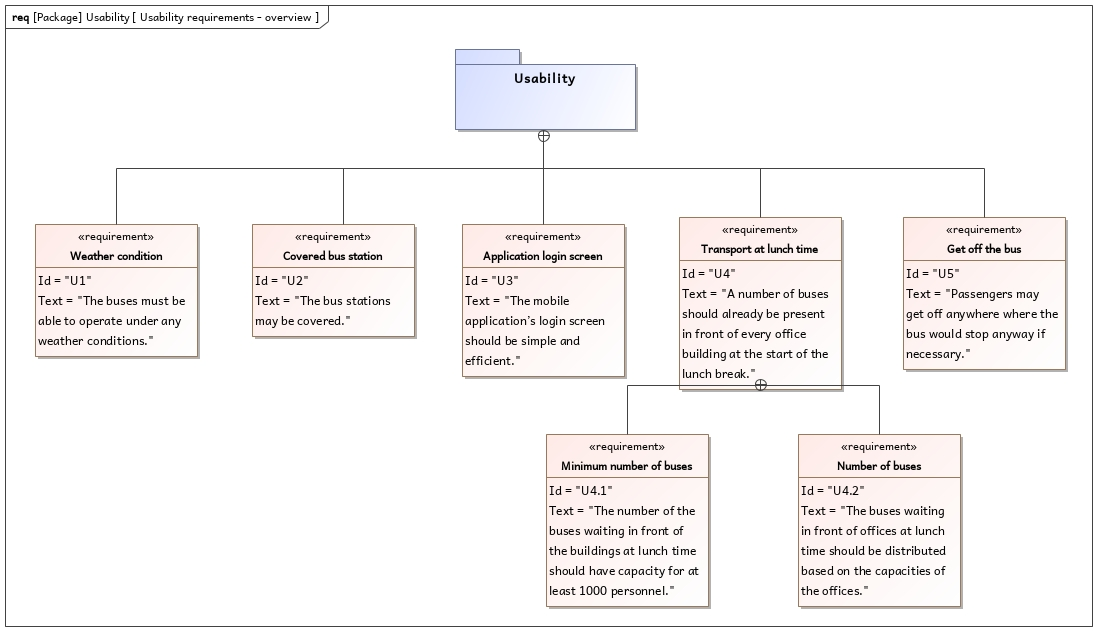
\includegraphics[width=\textwidth]{req-usability.jpg} % FIXME ugly
	\caption{Usability requirement diagram}%
	\label{fig:req-usability}
\end{figure}


% ------------------------------------------------------------------------------
\section{Use cases}

\begin{description}[style=nextline]
	\item[Make \gls{request} via \gls{mobileApplication}]
		Use the \gls{mobileApplication} designed especially for this
		system to make a \gls{request} for a lift. Only registered users
		may make \gls{request}s this way. The \gls{request} includes the
		user's identification, the date and time of the travel, their
		starting and destination point, as well as the number of people
		who wish to travel in case of a group \gls{request}.

	\item[Make \gls{request} via \gls{terminal}]
		Use the installed \gls{terminal}s in front of every office
		building to make a tranportation \gls{request}. When making a
		\gls{request} this way, only the travel destionation can—and
		must—be specified.

	\item[Monitor system status]
		Periodically check if the entire system is operating as
		expected—ie an appropriate number of buses is in operation (with
		regard to the number of users at the moment), the buses
		calculate \gls{route}s correctly and do not develop any faults.
		It must also be checked that the platforms for making
		\gls{request}s are fully operational.

	\item[Monitor bus condition]
		Keep watch on the various parameters of a bus to make sure it is
		functioning adequately.

	\item[Monitor bus position]
		Keep track of the positions of the buses to make sure they are
		located where they are supposed to be at any given time.

	\item[Avoid causing accidents]
		Ensure the buses cause harm to neither their environment nor
		their passengers. This is largely accomplished by collecting
		data from a variety of \gls{sensor}s and reacting in every
		situation intelligently, and handling unexpected occurrences.

	\item[Drive bus]
		Control the movement of a bus in order to fulfill the main
		purpose of the system: to transport passengers.

	\item[Find alternative \gls{route}]
		When a bus cannot run on a given \gls{route} (which can occur
		due to a variety of reasons) it must find an alternative
		\gls{route} to reach its destination provided such a path
		exists. The buses are aware of the road layout of the office
		park.

	\item[Select \gls{route}]
		The act of choosing a path between two locations in the office
		park, preferably the shortest.

	\item[Transport passengers]
		Get passengers to their desired destinations.

	\item[Manage \gls{request}s]
		Take \gls{request}s from users and use them to \gls{route} the
		buses in such a way that the \gls{request}s are carried out
		efficiently and quickly.

	\item[Monitor environment]
		The buses are aware of their surrounding area using several
		\gls{sensor}s installed for this purpose.

	\item[Notify mechanics]
		In case of a fault the bus ‘calls’ for repairs. Repairs can be
		made either remotely or manually. When possible, the buses
		return to the nearest \gls{terminal} where such repairs can be
		made.

	\item[Repair and maintain]
		Fix any potential problems with a bus and keep it in shape for
		continued usage.

	\item[Travel]
		Use the system to get from point A to point B.
\end{description}

\begin{figure}
	\centering
	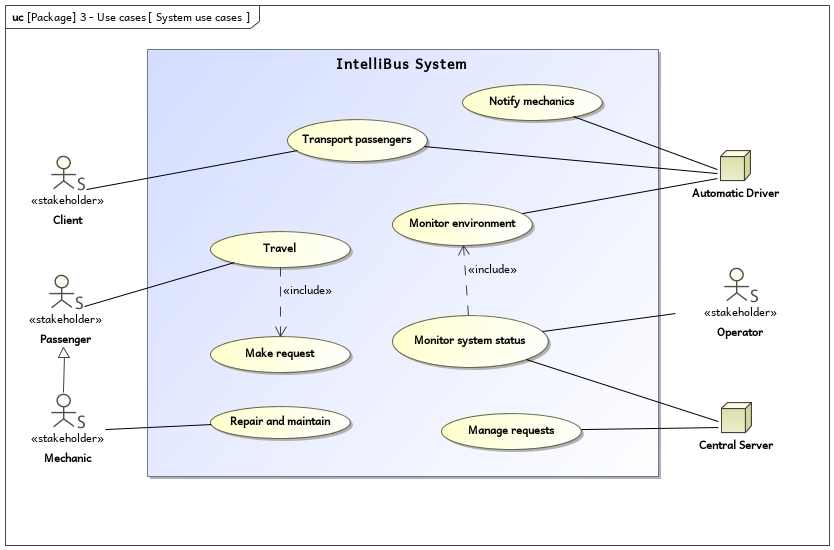
\includegraphics[width=\textwidth]{uc-system.jpg}
	\caption{System use cases}
\end{figure}


% ------------------------------------------------------------------------------
\section{Work journal}

\begin{tabularx}{\textwidth}{l l l X}
	\toprule
	Team member & Date & Time\footnote{in hours} & Activity \\ \midrule

	Borbála Szilágyi  & 2019-09-26 & 2   & meeting \\
	Bertalan Z. Péter & 2019-09-26 & 2   & meeting \\
	Annamária Gálik   & 2019-09-26 & 0.5 & collection of glossary items \\
	Borbála Szilágyi  & 2019-09-26 & 1   & collection of stakeholders \\
	Bertalan Z. Péter & 2019-09-26 & 0.5 & collection of system context
	                                       items \\
	Borbála Szilágyi  & 2019-09-27 & 1   & collection of requirements \\
	Annamária Gálik   & 2019-09-27 & 1   & extension of glossary \\
	Bertalan Z. Péter & 2019-09-27 & 1.5 & review, improvements, and a few
	                                       additional requirements \\
	Annamária Gálik   & 2019-09-27 & 1.5 & extension of glossary \\
	Borbála Szilágyi  & 2019-09-27 & 0.5 & impovements \\
	Annamária Gálik   & 2019-09-28 & 1   & extension of glossary,
	                                       improvement of definitions \\
	Borbála Szilágyi  & 2019-09-28 & 1   & detailed plan of the buses'
	                                       operation \\
	Bertalan Z. Péter & 2019-09-28 & 1   & improvement of requirements,
	                                       minor fixes, review \\
	Bertalan Z. Péter & 2019-09-28 & 0.5 & additional improvement and review
	                                       of requirements \\
	Borbála Szilágyi  & 2019-09-28 & 1   & diagram of stakeholders \\
	Borbála Szilágyi  & 2019-09-28 & 0.5 & functional requirements in
	                                       MagicDraw \\
	Annamária Gálik   & 2019-09-29 & 1   & new glossary terms, glossary in
	                                       MagicDraw \\
	Borbála Szilágyi  & 2019-09-29 & 1   & usability, security, and
					       dependability requirements in
					       Magic Draw \\
	Bertalan Z. Péter & 2019-09-29 & 2   & attempts at System Context
					       diagram; safety, performance, and
					       supportability requirements in
					       MagicDraw \\
	Bertalan Z. Péter & 2019-09-29 & 1   & LaTeX base document \\
	Annamária Gálik   & 2019-09-29 & 2   & our task, stakeholder, and work
					       journal in this document
					       (initial) \\
	Annamária Gálik   & 2019-09-30 & 2   & requirements and use cases in
	                                       this document \\
	Bertalan Z. Péter & 2019-09-30 & 1   & Context Diagram (final) \\
	Annamária Gálik   & 2019-09-30 & 3   & list of use cases, list of
					       requirements (also in this
					       document) \\
	Borbála Szilágyi  & 2019-09-30 & 2   & use case diagrams \\
	Borbála Szilágyi  & 2019-09-30 & 0.5 & context diagam improvements \\
	Bertalan Z. Péter & 2019-09-30 & 1   & descriptions of use cases \\
	Borbála Szilágyi  & 2019-09-30 & 0.5 & extensions of requirements \\
	Bertalan Z. Péter & 2019-10-01 & 1.5 & document formatting \\
	Bertalan Z. Péter & 2019-10-01 & 0.5 & review of this very document \\
	\bottomrule
\end{tabularx}

\clearpage
\printglossaries

\end{document}
